% !TeX encoding   = UTF-8
\documentclass[12pt]{article}

\usepackage{sbc-template}

\usepackage{graphicx,url}
\usepackage[brazil]{babel}
\usepackage[utf8]{inputenc}
\usepackage{graphicx}	%Package para figuras
\usepackage{enumerate}
\usepackage{tabularx}
\usepackage{multirow}
     
\sloppy

\title{Um Modelo para Predição da Confiabilidade\\
	  baseado em Métricas de Software}

%\author{Vagner Clementino\inst{1}}

\address{Departamento de Ciência da Computação\\
		Universidade Federal de Minas Gerais (UFMG)\\
%  \email{vagnercs@dcc.ufmg.br}
}

\begin{document} 

\maketitle

%\begin{abstract}
%  This meta-paper describes the style to be used in articles and short papers
%  for SBC conferences. For papers in English, you should add just an abstract
%  while for the papers in Portuguese, we also ask for an abstract in
%  Portuguese (``resumo''). In both cases, abstracts should not have more than
%  10 lines and must be in the first page of the paper.
%\end{abstract}
     
\begin{resumo} 
  A qualidade do software, apesar de ser um conceito abstrato, deve ser sempre buscada. Com a crescente complexidade dos sistemas fica cada vez mais difícil alcançar esta propriedade. Um fator chave para a qualidade do produto de software é a Confiabilidade. A Engenharia da Confiabilidade de Softwares é repleta de trabalhos que visam criar um modelo para medir a Confiabilidade. Seguinte esta tendência, este trabalho propõe a criação de um modelo estatístico capaz de mensurar a Confiabilidade de um software através de seus dados históricos de falhas, bem como de suas atuais métricas. Utilizando os dados coletados dos Bug Tracking System de cinco softwares de código aberto escritos em Java pretende-se confrontar as taxas de Confiabilidade obtidas com os bugs reportados na versão atual do sistema.
\end{resumo}


\section{Introdução}
\label{sec:intro}

A primeira preocupação no processo de desenvolvimento de um software é aderir o seu uso com os requisitos funcionais solicitados. Não obstante, a experiência mostra que os sistemas de sucesso são aqueles que não relegam ao segundo plano os requisitos não funcionais. Atributos não funcionais, tais como Adequação Funcional, Eficiência, Compatibilidade, Usabilidade, Confiabilidade, Segurança, Manutenibilidade e Portabilidade são características inerentes à \textit{qualidade} do produto de software\cite{citeulike:10951538}{}. Apesar do conceito de qualidade ser abstrato, deve-se sempre buscar formas de mensurá-lo e avaliá-lo.

De acordo com a ANSI, Software Confiabilidade é pode ser definida como a \textit{probabilidade} de operação de produto de software sem a ocorrência de falhas por um determinado \textit{período de tempo} em um ambiente específico \cite{IEEE-610.12-1990,pham2007system}{}. A Confiabilidade é um importante atributo da qualidade de software, todavia, é difícil de obter devido a intrínseca complexidade dos softwares. Analisando a definição de Confiabilidade, verifica-se que o conceito é visto como um função probabilística dependente do tempo. Esta definição remonta a origem  da área, que em seu início apresentava-se como uma especialização da tradicional Engenharia da Confiabilidade, cujo foco  estava na análise da durabilidade do hardware. Ao contrário do hardware, os softwares não sofrem a influência do tempo: um sistema com design ``perfeito'' que não sofra qualquer tipo de manutenção ou atualização irá executar sem falhas para sempre. Neste contexto, verifica-se que a principal diferença entre a Confiabilidade de Hardware e a de Software é que a segunda busca a perfeição design, ao  contrário da primeira que visa a perfeição da montagem/fabricação.

Desde o início da Engenharia de Software processos, ferramentas e metodologias vêm sendo criados com o objetivo de minimizar as falhas de softwares. Apesar de todo o esforço os problemas ainda persistem. A literatura é repleta de exemplos de problemas em softwares que acarretaram em prejuízos financeiros e até de perdas de vidas humanas. Um clássico exemplo é o Therac 25, uma máquina de terapia por radiação controlada por computador, que no ano de 1986 provocou graves lesões e mortes em pacientes devido a uma falha do seu software embutido. Cabe ressaltar que uma alta Confiabilidade não deveria ser uma preocupação apenas de aplicações críticas. A manutenção e evolução representa a maior parte dos custos do software\cite{1423995}{}, neste sentido garantir uma maior Confiabilidade representa redução de custos.

Apesar de sua importância, a Engenharia da Confiabilidade de Softwares ainda está dando os seus primeiros passos. Veremos na seção \ref{sec:problema} um dos problemas a serem resolvidos nesta área de pesquisa.
\section{O Problema a ser Resolvido}
\label{sec:problema}

Diferentemente de outras engenharias, o processo de mediação e avaliação dos softwares é ainda incipiente na Engenharia de Software. Questões como \textit{``Quão bom é um software, quantitativamente?"} ainda não produzem respostas satisfatórias. A fim de preencher esta lacuna diversos trabalhos vêm sendo propostos com objetivo de definir threshold de métricas de software\cite{rttool,csmrwcre2014b,5609747}, detectar bad smells\cite{7012985}{} e mensurar a Confiabilidade\cite{Lyu:1996,srm:2000}{}.

Os trabalhos relacionados à predição da Confiabilidade de Software podem ser divididos entre os de \textit{Modelos de Predição} e os dos \textit{Modelos de Estimação}{}\cite{Lyu:2007:SRE:1253532.1254716}{}. O primeiro grupo têm por objetivo predizer a Confiabilidade em algum ponto do futuro com base em dados históricos. O segundo visa estimar a Confiabilidade no presente ou em algum ponto futuro utilizando dados atuais do processo de desenvolvimento de software.

Apesar da grande contribuição dos trabalhos de predição da Confiabilidade, não há um modelo que atenda todas as situações. Devido à complexidade do inerente ao software, qualquer modelo de predição naturalmente necessitar de algum pressuposto adicional. Ademais, existem poucos trabalhos que consideram métricas de medição de software, tais como \textsc{Depth of Inheritance Tree (DIT), Number of Children (NOC), Coupling between Object Classes (CBO), Lack of Cohesion of Methods (LCOM), Weighted Methods per Class (WMC)}, no processo de predição da Confiabilidade. 

\section{Solução Proposta}
\label{sec:proposta}

Este documento propõe um estudo com o objetivo de formular um modelo estatístico que possibilite mensurar a Confiabilidade de software utilizando dados históricos, bem como suas respectivas métricas de software. A taxa de confiabilidade será data ao nível de um módulo de software. Neste trabalho, entende como módulo a separação lógica de funcionalidades do sistema.

A fim de calcular a taxa de Confiabilidade dos sistemas, pretende-se coletar dados de falhas de cinco programas de código aberto escritos em Java. Os dados serão coletados diretamente do \textit{Bug Tracking System - BST}{} da aplicação. De posse dos dados de falhas, será coletados as métricas dos softwares. Posteriormente será calculado a taxa de confiabilidade de cada um dos módulos que compõem o sistema. O cálculo ao nível de um módulo, se deve essencialmente pelo dificuldade em conseguir dados de bugs em uma menor granularidade, como por exemplo ao nível de classes ou \textit{packages}{}. Estudos estão sendo realizados com o objetivo de definir o melhor modelo estatístico a ser aplicado no calculo da Confiabilidade. Um outro ponto em aberto neste trabalho é quanto a escolha da ferramente para coleta das métricas de software.

\section{Trabalhos Relacionados}
\label{sec:trab_relacionados}


\section{Solução Proposta}
\label{sec:proposta}

\section{Avaliação do Modelo}
\label{sec:avaliacao}

\subsection{Coleta e Análise dos Bugs}
\label{subsec:analise_coleta_bugs}

A fim de avaliar o modelo proposto foram coletados os dados de bugs de quatro sistemas implementados em Java e desenvolvidos pela Apache Software Foundation\footnote{\url{http://www.apache.org}}. A Tabela \ref{tab:sistemas} exibe algumas informações dos softwares utilizados. Os sistemas foram escolhidos por possuírem uma base de usuários abrangente e ativa, além de possuírem um grande número de bugs registrados no BST da Apache Foundation. Tomou-se também o cuidado de escolher sistemas de diferentes categorias de software com objetivo de reduzir algum viés resultante do uso do mesmo tipo de aplicação.

\begin{table}[h]
\resizebox{\textwidth}{!}{%
\begin{tabular}{|l|l|l|c|}
\hline
\multicolumn{1}{|c|}{{\bf Produto}} & \multicolumn{1}{c|}{{\bf Descrição}} & \multicolumn{1}{c|}{{\bf Categoria}} & {\bf KLOC} \\ \hline
\textit{Ant} & Ferramenta utilizada para automação de compilação de software. & Gerenciamento da Compilação & ??? \\ \hline
\textit{JMeter} & Ferramenta utilizada para testes de carga em um servidores, redes ou objetos Java. & Ferramenta de Testes & ??? \\ \hline
\textit{Log4j} & API para que o desenvolvedor de software possa fazer log de dados na aplicação. & Biblioteca & ??? \\ \hline
\textit{Tomcat 7} & Servidor web Java que implementa as tecnologias Java Servlet e JavaServer Pages. & Servidor Web & ??? \\ \hline
\end{tabular}
}
\caption{Sistemas utilizados na avaliação}
\label{tab:sistemas}
\end{table}

Os erros em sistemas da Apache Foundation podem ser reportados através da ferramenta ASF Bugzilla\footnote{\url{https://bz.apache.org/bugzilla/}}{}. Com objetivo de recuperar as informações dos bugs dos sistemas constantes da Tabela \ref{tab:sistemas} foi criado desenvolvido uma aplicação, denominada \textit{ASFBugScraper}, que recupera os dados de um bug diretamente da página html do ASF Bugzilla. Este tipo de processo é conhecido como \textit{web scraping}. Inicialmente foi coletado de forma manual do site ASF Bugzilla uma lista no formato \textit{.csv} com todos os bugs para um determinado sistema\footnote{Bugs registrados até 04/06/2015}. Esta lista contêm apenas informações básicas sobre os erros reportados, contudo, possui o \textit{id} do bug (identificador único dentro do ASF Bugzilla), o que possibilitava que as demais informações do bug fossem recuperadas. A partir desta lista de bugs foi realizada uma coleta de dados utilizando a ferramenta \textit{ASFBugScraper}. Para cada bug foi recuperados os dados constante da Tabela \ref{tab:campos}{}.

\begin{table}[h]
\resizebox{\textwidth}{!}{%
\begin{tabular}{|l|l|}
\hline
\multicolumn{1}{|c|}{{\bf Campo}} & \multicolumn{1}{c|}{{\bf Descrição}}                                                             \\ \hline
\textit{ID}                                & Identificador de um bug no ASF Bugzilla                                                          \\ \hline
Situação                          		  & Identifica o estado atual de um bug.                                                             \\ \hline
\textit{Produto}                           & O sistema no qual o bug ocorreu                                                                  \\ \hline
\textit{Versão}                            & A versão do sistema em que o bug ocorreu                                                         \\ \hline
\textit{Componente}                        & Identifica o módulo do sistema em que o bug ocorreu                                              \\ \hline
\textit{Hardware}                          & A plataforma de hardware no qual o erro foi observado.                                           \\ \hline
\textit{Importância}                       & A importância de um bug é descrita como a combinação de sua prioridade e gravidade.              \\ \hline
\textit{Target Milestone}                  & O campo   Target Milestone identifica em qual versão do sistema o bug deverá estar selecionado. \\ \hline
\textit{Atribuído Para}                    & Identifica o responsável pela resolução do bug.                                                   \\ \hline
\textit{Data do Bug}                       & Contêm a data em que o bug foi reportado.                                 \\ \hline
\textit{Relatado Por}                      & Identifica o responsável por informar o bug.                                                      \\ \hline
\textit{Data da Ultima Alteração}          & Contêm a data da última alteração ocorrida na resolução do bug. \\ \hline
\textit{Descrição do Bug}                  & Contêm os detalhes do problema reportado.                                                         \\ \hline
\end{tabular}
}
\caption{Campos recuperados pelo \textit{ASFBugScraper}}
\label{tab:campos}
\end{table}

Para fins da validação do modelo proposto foram considerados apenas os bugs cuja situação seja \textit{``CONFIRMED"}, \textit{``RESOLVED-FIXED"}, \textit{``RESOLVED-WONTFIX"}, \textit{``VERIFIED-FIXED"} e \textit{``VERIFIED-WONTFIX"}\footnote{Para maiores detalhes vide \url{https://bz.apache.org/bugzilla/page.cgi?id=fields.html#bug_status}}. Um bug na situação \textit{``CONFIRMED"} foi verificado como válido por alguns dos desenvolvedores a Apache Foundation. As situações \textit{``RESOLVED-FIXED"} e  \textit{``RESOLVED-WONTFIX"} representam bugs  confirmados e resolvidos; sendo que no primeiro caso uma solução foi desenvolvida e testada; o segundo representa bugs que nunca serão resolvidos. Os erros nas situações \textit{``VERIFIED-FIXED"} e \textit{``VERIFIED-WONTFIX"} foram confirmados e verificados pelo setor qualidade (\textit{QA}) da Apache Foundation. A partir deste filtro é possível remover bugs inválidos, duplicados ou cujo erro não pode ser reproduzidos nos teste do desenvolvedor. Em síntese, apenas erros efetivamente confirmados serão analisados.

Os bugs foi divididos em duas categorias \textsc{CAT-HIST} e \textsc{CAT-LAST}. Dado um sistema $S$ composto pelos módulos $M_1, M_2$ e $M_3$, no qual cada um dos módulo está presente nas versões $v_0, v_1 \ldots v_n$ do software.  Seja $B_i$ o conjunto de bugs coletados na versão $v_i$ do sistema, onde $0 \leq i \leq n${}. Para cada módulo de $S$, os bugs pertencentes à $B_0, B_1, \ldots, B_{(n-1)}$  estarão na categoria \textsc{CAT-HIST}. Estes dados serão utilizados para de calcular a taxa de confiabilidade $\omega$ do módulo. Naturalmente os bugs em $B_n$ estão na categoria \textsc{CAT-LAST}. A partir dos valores obtido de $\omega$ foi realizado uma comparação com os bugs em \textsc{CAT-LAST}. A Figura \ref{fig:avalicao} exibe de forma abstrata o processo de avaliação. Na tabela temos as versões e o tamanho de amostra em cada uma das categorias para os sistema utilizado na avaliação.

\begin{figure}[ht]
\centering
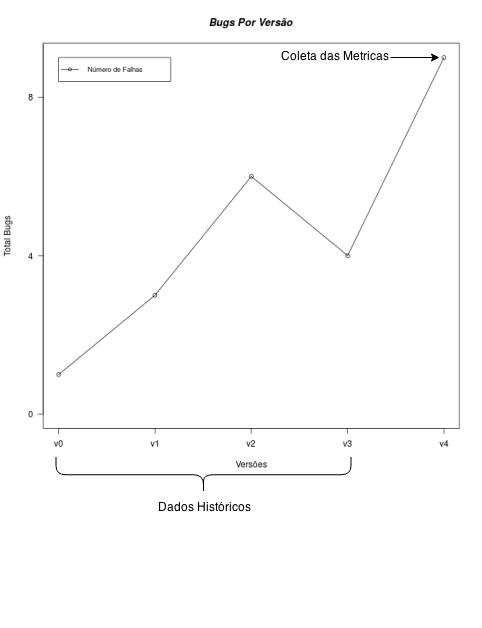
\includegraphics[width=.80\textwidth]{./img/projeto_mes_avaliacao.png}
\caption{Processo de Avaliação: Visão abstrata}
\label{fig:avalicao}
\end{figure}

\subsection{Coletando as métricas}
\label{subsec:analise_coleta_metricas}

\section{Resultados}
\label{sec:resultados}
\section{Limitações e Ameaças a Validade}
\label{sec:limitacoes}

Uma primeira limitação deste trabalho está no fato de não ser possível de medir a taxa de Confiabilidade em uma granularidade menor do que um módulo. Conforme exposto, é difícil encontrar informações sobre bugs ao nível de classe ou package. Um outro fator limitador está relacionado ao número de sistemas avaliados bem como a linguagem utilizado. O fato de usar um número reduzido de sistemas desenvolvidos em uma mesma linguagem dificulta a generalização dos resultados obtidos. Por se tratar de um modelo estatística para o cálculo da Confiabilidade, simplificações e outras suposições são necessárias. Todavia, está é uma ameaça comum a validade de qualquer trabalho nesta área.

\section{Conclusão}
\label{sec:conclusao}

\bibliographystyle{sbc}
\bibliography{./bib/proposta-ref}

\end{document}
